% fancytikzposter.tex, version 2.1
% Original template created by Elena Botoeva [botoeva@inf.unibz.it], June 2012
% 
% This file is distributed under the Creative Commons Attribution-NonCommercial 2.0
% Generic (CC BY-NC 2.0) license
% http://creativecommons.org/licenses/by-nc/2.0/ 

\documentclass{a0poster}

%\usepackage[T1]{fontenc}
%\usepackage[latin9]{inputenc}
\usepackage{fancytikzposter} 


%%%%% --------- Change here if you want ---------- %%%%%
%% margin for the geometry package, must be changed before using the geometry package
%% default value is 4cm
\setmargin{1.2}

%% the space between the blocks
%% default value is 2cm
% \setblockspacing{2}

%% the height of the title stripe in block nodes, decrease it to save space
%% default value is 3cm
% \setblocktitleheight{3}

%% the number of columns in the poster, possible values 2,3
%% default value is 2
% \setcolumnnumber{3}

%% the space between two or more groups of authors from different institutions
%% used in \maketitle
% \setinstituteshift{10}

%% which template to use
%% N1 simple, standard look, with a colored background and gray boxes
%% N2 board with nodes
%% N3 another standard look
%% N4 envelope-like look
%% N5 with a wave-like head, original idea taken from
%%%% http://fc09.deviantart.net/fs71/f/2010/322/1/1/scientific_poster_by_nabuy-d333ria.jpg
%\usetemplate{4}
\usetemplate{2}


%% components of the templates
%% (the maximal possible numbers are mentioned as the parameters)
% \usecolortemplate{4}
% \usebackgroundtemplate{4}
%\usetitletemplate{2}
%\usetitletemplate{2}

%\useblocknodetemplate{4}
% \useplainblocktemplate{4}
% \useinnerblocktemplate{2}


%% the height of the head drawing on top 
%% applicable to templates N3, 4 and 5
% \setheaddrawingheight{14}


%% change the basic colors
%\definecolor{myblue}{HTML}{008888} 
%\setfirstcolor{myblue}% default 116699
%\setsecondcolor{gray!80!}% default CCCCCC
%\setthirdcolor{red!80!black}% default 991111

%% change the more specific colors
% \setbackgrounddarkcolor{colorone!70!black}
% \setbackgroundlightcolor{colorone!70!}
% \settitletextcolor{textcolor}
% \settitlefillcolor{white}
% \settitledrawcolor{colortwo}
% \setblocktextcolor{textcolor}
% \setblockfillcolor{white}
% \setblocktitletextcolor{colorone}
% \setblocktitlefillcolor{colortwo} %the color of the border
% \setplainblocktextcolor{textcolor}
% \setplainblockfillcolor{colorthree!40!}
% \setplainblocktitletextcolor{textcolor}
% \setplainblocktitlefillcolor{colorthree!60!}
% \setinnerblocktextcolor{textcolor}
% \setinnerblockfillcolor{white}
% \setinnerblocktitletextcolor{white}
% \setinnerblocktitlefillcolor{colorthree}



%%% size of the document and the margins
%% A0
% \usepackage[margin=\margin cm, paperwidth=118.9cm, paperheight=84.1cm]{geometry} 
\usepackage[margin=\margin cm, paperwidth=84.1cm, paperheight=118.9cm]{geometry}
%% B1
% \usepackage[margin=\margin cm, paperwidth=70cm, paperheight=100cm]{geometry}



%% changing the fonts
\usepackage{cmbright}
%\usepackage[default]{cantarell}
%\usepackage{avant}
%\usepackage[math]{iwona}
\usepackage[math]{kurier}
\usepackage[T1]{fontenc}
\usepackage[utf8]{inputenc}



%% add your packages here
\usepackage{hyperref}
\usepackage{xcolor}
\usepackage{graphicx}

%\usepackage{subfiles}
\usepackage{standalone}


\usepackage{color}
\usepackage{wrapfig}
\usepackage{graphicx}
\usepackage{nomencl}

\title{Keyword Search over Data Service Integration for Accurate Results}
%\qquad version 2.1
\author{Vidmantas Zemleris\\
%  Faculty of Mathematics and Informatics\\
   Vilnius University, Lithuania\\
   %(at CMS Experiment, CERN)\\
  \texttt{vidmantas.zemleris@cern.ch}\\
  for the benefit of CMS Collaboration
  \And
  Valentin Kuznetsov\\
  Cornell University, USA\\
  \texttt{vkuznet@gmail.com}
  \newline
}



%%%%%%%%%%%%%%%%%%%%%%%%%%%%%% LyX specific LaTeX commands.
%% The greyedout annotation environment

\usepackage{color}
\definecolor{note_fontcolor}{rgb}{0.5, 0.5, 0.5}
\definecolor{grey_dark}{rgb}{0.7, 0.7, 0.7}
%\definecolor{grey_dark}{rgb}{0.6, 0.6, 0.7}
\definecolor{grey_light}{rgb}{0.9, 0.9, 0.9}

\newenvironment{lyxgreyedout}
  {\textcolor{note_fontcolor}\bgroup\ignorespaces}
  {\ignorespacesafterend\egroup}
%% A simple dot to overcome graphicx limitations
\newcommand{\lyxdot}{.}

\usepackage[english,british]{babel}

\usepackage{textcomp}

\begin{document}

\newcommand{\note}{}

%\newcommand{\skip1@preamble}{%
% \let\document\relax\let\enddocument\relax%
% \let\usepackage\relax%
% \newenvironment{document}{}{}%
% \renewcommand{\documentclass}[2][subfiles]{}}
% \newcommand\subfile[1]{\begingroup\skip1@preamble\input{#1}\endgroup}


%%%%% ---------- the background picture ---------- %%%%%
%% to change it modify the macro \BackgroundPicture
\ClearShipoutPicture
\AddToShipoutPicture{\BackgroundPicture}

\noindent % to have the picture right in the center
\begin{tikzpicture}
  \initializesizeandshifts
  % \setxshift{15}
  \setyshift{1.5}


  %% the title block, #1 - shift, the default value is (0,0), #2 - width, #3 - scale
  %% the alias of the title block is `title', so we can refer to its boundaries later
  \ifthenelse{\equal{\template}{1}}{ 
    \titleblock{70}{1.0}
  }{
    %\titleblock{47}{1.5}	
        \titleblock{75}{1.0}

  }

  %% a logo can be added to the title block
  %% #1 - anchor relative to the title block, #2 - shift, #3 - width, #3 - file name
  % \ifthenelse{\equal{\template}{2}}{ 
  %   \addlogo[south west]{(2,0)}{6cm}{unibz_b.png}
  % }{
  %   \addlogo[south west]{(2,0)}{6cm}{unibz_w.png}
  % }
  \addlogo[south west]{(0,-1.5)}{6cm}{images/vu_logo.png}
  \addlogo[south west]{(7,-1.5)}{6cm}{images/mif.png}
	%
  \addlogo[south east]{(0,-1.5)}{6cm}{images/cern_logo.png}
  \addlogo[south east]{(-7,-1.5)}{6cm}{images/cms_logo.png}



  %% a block node, with the specified position (optional), title and the content
  %% #1 - where (optional), #2 - title, #3 - text
  %%%%%%%%%% ------------------------------------------ %%%%%%%%%%
%  \getcurrentrow{box}
  %\blocknodew[(0, 45)]{75}%
  \blocknode%
  {Summary}%
  {%
  %\textbf{Background:} 
  Virtual data integration aims at providing a coherent interface for querying heterogeneous data sources (e.g. web services, proprietary systems) with minimum upfront effort in integration. %
  %This work explores various aspects of its usability.
Data is usually accessed through a structured queries, such as SQL, requiring to learn the language and to get acquainted with data organization, which may pose problems even to proficient users.
% thus negatively impacting the system’s usability.%

%\note{, given a keyword query,}
%\textbf{Solution:} 
\quad We present a keyword search system, which proposes a ranked list of structured queries along with their explanations. It operates mainly on the metadata, such as the constraints on inputs accepted by services.
%{\color{red}, analysis of user queries, and only certain portions of the data.} %
% nlike previous implementations,
% and makes no assumptions about the input query, while maintaining its ability to leverage the query’s structural patterns - in case they exist.}%
It was developed as an integral part of the CMS data discovery service 
	% {\color{red} focusing on simplicity and capabilities of the interface},
	 and is currently available as open source.
%{\color{red}The system is }.
}


  %% a callout block
  %% #1 - rotate angle (optional), #2 - from, #3 - where, #4 - width, #5 - text
  %%%%%%%%%% ------------------------------------------ %%%%%%%%%%
%  \calloutblock{($(box.center)+(-2,-8)$)}
%  {($(box.center)+(10,-1)$)}
%  {19cm}
%  {\small
%    Macro for creating a block node:
%    \begin{itemize}
%    \item[] \textbackslash blocknode\{Block Title\}\{Block Content\}
%    \end{itemize}
%    Macro \textbackslash blocknode has three parameters. The first one is
%    optional and it is the position of the block. The first block will be
%    automatically placed to (\$(firstrow)-(xshift)-(yshift)\$), which is the
%    left corner below the title block. In most of the templates, (firstrow) is
%    set to (title.south), where \emph{title} is the alias for the title
%    block. Each subsequent block is automatically placed to
%    [(\$(box.south)-(yshift)\$)], i.e., below the previous block aliased
%    \emph{box}.  You can also use an explicit parameter, e.g., $(-10,30)$ (note
%    that (0,0) is the center of the poster). The second parameter is the title
%    of the block. Finally, the last parameter is the  actual content. 
%  }




  %% by default, the position of the new block node is right below the previous
  %% block node, stored in (currenty)
  %% box is the alias of the previous block, so we can refer to its boundaries

  %%%%%%%%%% ------------------------------------------ %%%%%%%%%%
  \blocknode{Context: a system for Virtual Data Integration}%
  {%
  %% LyX 2.0.6 created this file.  For more info, see http://www.lyx.org/.
%% Do not edit unless you really know what you are doing.
\documentclass{standalone}
\usepackage{graphicx}

\makeatletter

%%%%%%%%%%%%%%%%%%%%%%%%%%%%%% LyX specific LaTeX commands.
%% A simple dot to overcome graphicx limitations
\newcommand{\lyxdot}{.}


\makeatother

\begin{document}
\begin{wrapfigure}{r}[0.1\columnwidth]{0.6\columnwidth}% 
\vspace{-40pt}\hspace{-1cm}
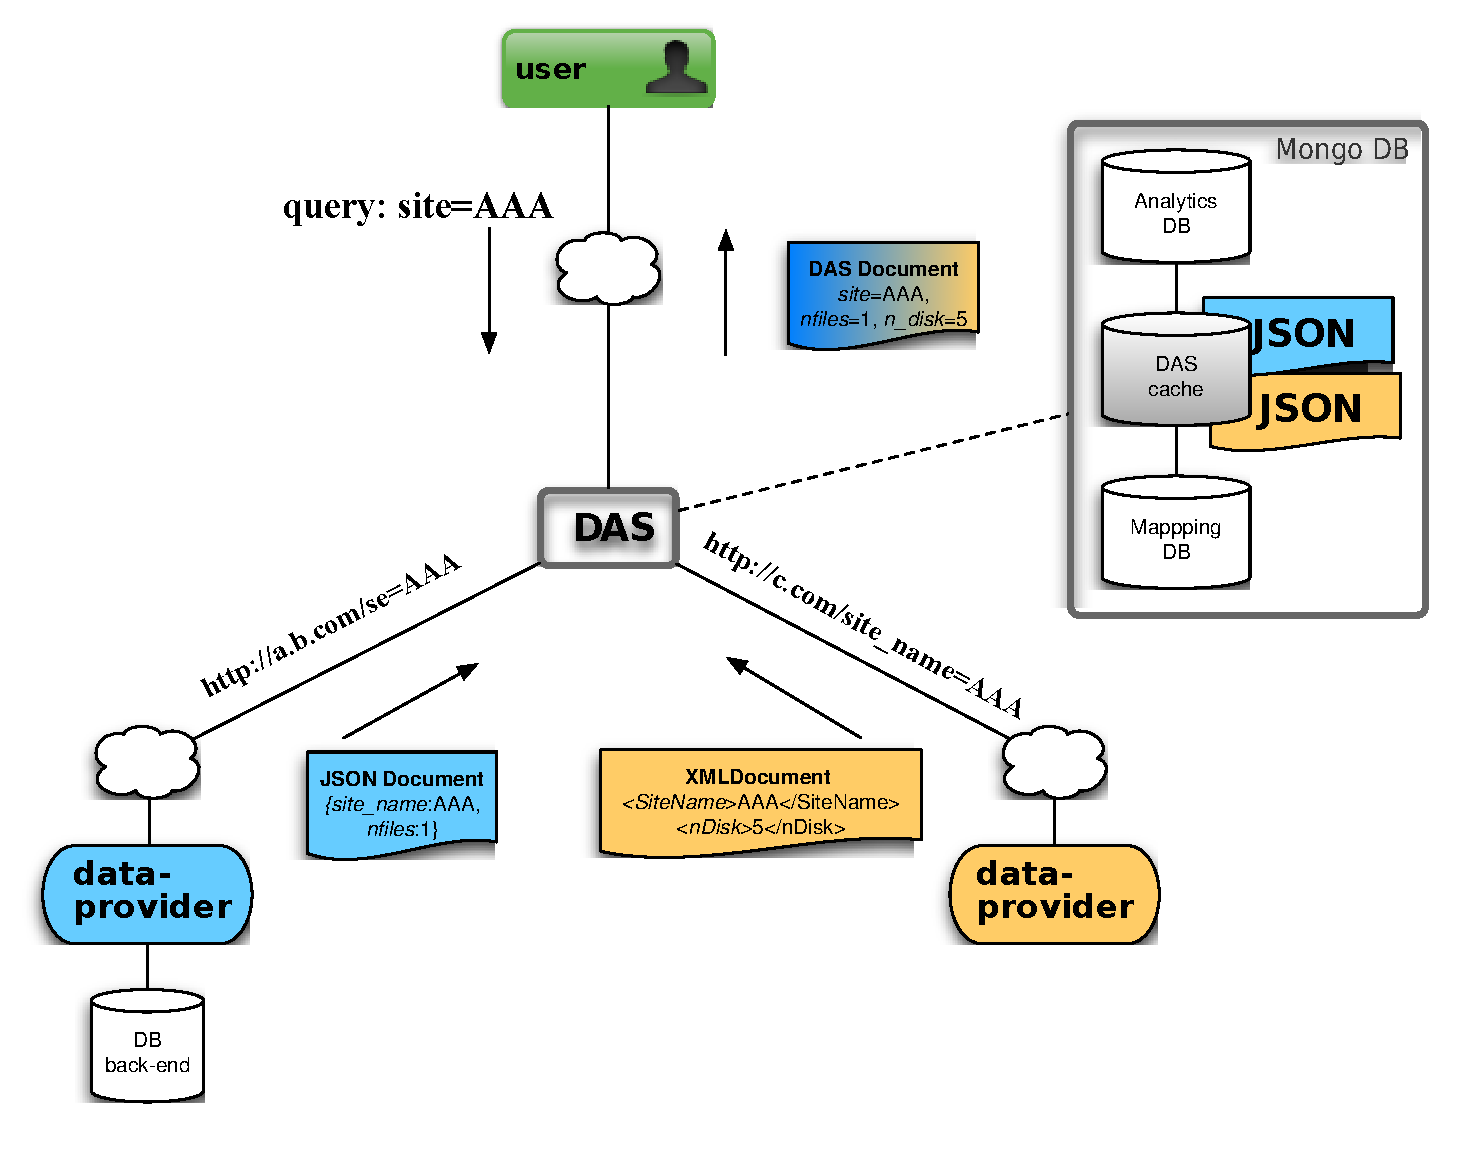
\includegraphics[width=0.55\columnwidth]{images/das}
\vspace{-2.5cm}
\caption{DAS workflow}
\vspace{-4cm}
\end{wrapfigure}% 

\textbf{''CMS Data Aggregation System'' (DAS):}
\begin{itemize}
\item accepts simple structured queries
\item integrates heterogeneous services

\begin{itemize}
\item parse the query \& contact services
\item eliminate inconsistencies in responses:

\begin{itemize}
\item entity naming
\item data formats {\footnotesize{(XML, JSON)}}{\footnotesize \par}
\end{itemize}
\item combine them
\end{itemize}
\item requires only minimal service mappings

\begin{itemize}
\item no predefined schema
\item minimal effort in defining services
\end{itemize}
\end{itemize}

\paragraph{Queries}

must specify: entity to be retrieved and filtering criteria. Optionally,
the results can be further filtered, sorted or aggregated

\includegraphics[width=1\textwidth]{/home/vidma/DAS_paper/figures/DASQL_structure}
\end{document}
%
  }
  \plainblock[3]{($(box.south)+(3,1)$)}{30}%
  {\vspace{-20pt}\newline%
    still, it is overwhelming for users to:}%
  {%\vspace{-10pt}
  \begin{itemize}
  	\item learn the query language
	\item remember how exactly the data is structured and named 
  \end{itemize}
  \textbf{\textit{Could keyword queries solve this?}}%
  \vspace{-20pt}}
  
  \getcurrentrow{note}
  \coordinate (currenty) at ($(currentrow)-(yshift)-(xshift)+(0,0.5)$);


  %%%%%%%%%% ------------------------------------------ %%%%%%%%%%
  \blocknode{Interpreting Keyword Queries: Problem definition} %
  {%
    %% LyX 2.0.6 created this file.  For more info, see http://www.lyx.org/.
%% Do not edit unless you really know what you are doing.
\documentclass{standalone}
\usepackage{wrapfig}
\usepackage{graphicx}
\usepackage{nomencl}
% the following is useful when we have the old nomencl.sty package
\providecommand{\printnomenclature}{\printglossary}
\providecommand{\makenomenclature}{\makeglossary}
\makenomenclature

\makeatletter

%%%%%%%%%%%%%%%%%%%%%%%%%%%%%% LyX specific LaTeX commands.
%% A simple dot to overcome graphicx limitations
\newcommand{\lyxdot}{.}


\makeatother

\begin{document}
\begin{wrapfigure}{o}{0.4\textwidth}%
\vspace{-40pt}

\includegraphics[width=0.4\textwidth]{/home/vidma/DAS_paper/figures/problem_statement_das_service_ex}\vspace{-20pt}\caption{a data-service (simplified)}
\end{wrapfigure}%


\textbf{Input:} query, KWQ\nomenclature{KWQ}{keyword query\\}=$\left(kw_{1},kw_{2},..,kw_{n}\right)$

\textbf{Task: }translate it into structured query

\textbf{Given: }metadata
\begin{itemize}
\item names of entities and their attributes 

\begin{itemize}
\item (either \emph{service inputs} or their \emph{output} fields)
\end{itemize}
\item possible values (only for some inputs)
\item \emph{constraints} on data-service \emph{inputs}:

\begin{itemize}
\item mandatory inputs
\item regular expressions on values\end{itemize}
\end{itemize}

\end{document}

  }
  %%%%%%%%%% ------------------------------------------ %%%%%%%%%%

  \setplainblockfillcolor{grey_light}
  \calloutblock[4]{($(box.center)+(10,6)$)}%
  		{($(box.south east)+(-11,10)$)}{23} %
  {%    
    \vspace{0.3cm}
    %% LyX 2.0.6 created this file.  For more info, see http://www.lyx.org/.
%% Do not edit unless you really know what you are doing.
\documentclass{standalone}
\usepackage{color}
\usepackage{graphicx}

\makeatletter

%%%%%%%%%%%%%%%%%%%%%%%%%%%%%% LyX specific LaTeX commands.
%% A simple dot to overcome graphicx limitations
\newcommand{\lyxdot}{.}


\makeatother

\begin{document}
\textbf{Example. }Consider these queries: 
\begin{itemize}
\item average\textcolor{red}{{} }size of RelVal datasets with number of events
more than 1000
\item avg dataset size RelVal number of events\textgreater{}1000
\item avg(dataset size) RelVal `number of events'\textgreater{}1000
\end{itemize}
For all, the expected result is:

\includegraphics[width=1\textwidth]{/home/vidma/DAS_paper/figures/DASQL_1avg_problem_statement}


\end{document}
%
    }
  %% the coordinate (currenty) is used in the default placing of the next blocknode
  %\getcurrentrow{note}
  \getcurrentrow{note}
  %\coordinate (currenty) at ($(currentrow)-(yshift)-(xshift)+(0,2)$);
  \coordinate (currenty) at ($(currentrow)-(yshift)-(xshift)+(0,0)$);


  %%%%%%%%%% ------------------------------------------ %%%%%%%%%%
  \blocknode%
  {Keyword search overview}%
  {
	%% LyX 2.0.6 created this file.  For more info, see http://www.lyx.org/.
%% Do not edit unless you really know what you are doing.
\documentclass{standalone}
\usepackage{color}
\definecolor{note_fontcolor}{rgb}{0.80078125, 0.80078125, 0.80078125}
\usepackage{graphicx}

\makeatletter

%%%%%%%%%%%%%%%%%%%%%%%%%%%%%% LyX specific LaTeX commands.
%% The greyedout annotation environment
\newenvironment{lyxgreyedout}
  {\textcolor{note_fontcolor}\bgroup\ignorespaces}
  {\ignorespacesafterend\egroup}
%% A simple dot to overcome graphicx limitations
\newcommand{\lyxdot}{.}


\makeatother

\begin{document}
\selectlanguage{english}%
\begin{center}
\begin{minipage}[t]{0.5\columnwidth}%
\begin{itemize}
\item tokenizer:

\begin{itemize}
\item clean up the query
\item identify patterns
\end{itemize}
\item identify and score ``\emph{entry points}'' with

\begin{itemize}
\item string matching %
\begin{lyxgreyedout}
{[}for entity names{]}%
\end{lyxgreyedout}

\item IR (IDF-based) %
\begin{lyxgreyedout}
 {[}output fieldnames{]}%
\end{lyxgreyedout}

\item list of known values
\item regular expressions on allowed values
\end{itemize}
\item combine\emph{ entry points}

\begin{itemize}
\item consider various \emph{entry point} permutations %
\begin{lyxgreyedout}
 (keyword labelings)%
\end{lyxgreyedout}

\item promote ones respecting keyword dependencies or other heuristics
\item interpret as structured queries \selectlanguage{english}%
\end{itemize}
\end{itemize}
%
\end{minipage}\,%
\begin{minipage}[t]{0.4\columnwidth}%
\selectlanguage{british}%
\textbf{\vspace{-80pt}}

\textbf{\includegraphics[width=0.99\textwidth]{/home/vidma/DAS_paper/figures/DAS_KWS_architecture}}\selectlanguage{english}%
%
\end{minipage} 
\par\end{center}\selectlanguage{british}%

\end{document}

  }
  %% to place the next node centered vertically in the second column, we can
  %% obtain the y-coordinate of the previous node using macro
  %% \getcurrentrow{note}, where note is the alias of the callout node, and
  %% then specify the coordinate of the next node using coordinate (currentrow)
  \getcurrentrow{box} 
  \coordinate (kws_north) at ($(box.north)$);
  \coordinate (kws_overv) at ($(box.south east)$);  

  \plainblock[0]{($(box.south west)-(yshift)-(-3,0)$)}%
  {8cm}{} %
  {\newline\vspace{-0cm}
  	\textbf{More info:}\vspace{0.5cm}
  	\newline
    
\includegraphics[width=5cm]{images/qrcode.png}
  	\vspace{-0cm}
  }  
  
  %% a plain block
  %% #1 - rotate angle (optional), #2 - where, #3 - width, #4 - title, #5 - text
  %%%%%%%%%% ------------------------------------------ %%%%%%%%%%
  \setplainblockfillcolor{white}
  \calloutblock[0]{($(kws_overv)+(-4.9,2.7)$)}%
  		{($(box.south east)-(yshift)+(-14, 0)$)} %
  {27} %
  {
  %\textbf{\color{blue}Result presentation:}
  %\newline
  	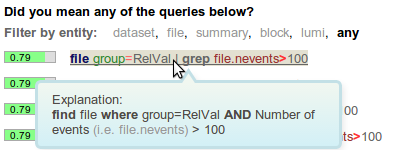
\includegraphics[width=1.0\textwidth]{ui_result.png}
  	\vspace{-50pt}
  }
  
  \getcurrentrow{note}
  \coordinate (currenty) at ($(currentrow)+(yshift)$);

  %% the coordinate (currenty) is used in the default placing of the next blocknode
 %\getcurrentrow{note}
 %\coordinate (currenty) at ($(currentrow)+(xshift)-(yshift)$);





  %%%%%%%%%%%%% NEW COLUMN %%%%%%%%%%%%%%% 
  \startsecondcolumn 

  %%%%%%%%%% ------------------------------------------ %%%%%%%%%%
  \blocknode%
  {Challenges}%
  {
	%% LyX 2.0.6 created this file.  For more info, see http://www.lyx.org/.
%% Do not edit unless you really know what you are doing.
\documentclass{standalone}
\usepackage{color}
\definecolor{note_fontcolor}{rgb}{0.80078125, 0.80078125, 0.80078125}
\usepackage{textcomp}

\makeatletter

%%%%%%%%%%%%%%%%%%%%%%%%%%%%%% LyX specific LaTeX commands.
%% The greyedout annotation environment
\newenvironment{lyxgreyedout}
  {\textcolor{note_fontcolor}\bgroup\ignorespaces}
  {\ignorespacesafterend\egroup}

\makeatother

\begin{document}
\begin{itemize}
\item queries are ambiguous

\begin{itemize}
\item return ranked list of structured query suggestions
\end{itemize}
\item no direct access to the data

\begin{itemize}
\item querying services is expensive \textrightarrow{} rely on metadata
\item bootstrap list of allowed values %
\begin{lyxgreyedout}
(available only for some fields) %
\end{lyxgreyedout}

\item rely on \emph{regexps} with lower confidence %
\begin{lyxgreyedout}
(can result in false positives)%
\end{lyxgreyedout}

\end{itemize}
\item no predefined schema

\begin{itemize}
\item bootstrap list of fields in service results through queries
\item some field names are unclean \textrightarrow{} use IDF %
\begin{lyxgreyedout}
(as they come directly from JSON/XML responses)%
\end{lyxgreyedout}
\end{itemize}
\end{itemize}

\end{document}

  }


  %%%%%%%%%% ------------------------------------------ %%%%%%%%%%
  

  \setinnerblocktitlefillcolor{grey_dark}

  \blocknode%
  {The ranker}%
  {
	%% LyX 2.0.6 created this file.  For more info, see http://www.lyx.org/.
%% Do not edit unless you really know what you are doing.
\documentclass{standalone}
\begin{document}
\selectlanguage{english}%
\[
score\_prob=\sum_{i=1}^{|KWQ|}\left({\displaystyle {\displaystyle \ln}\left(score(tag_{i}|kw_{i})\right)}+\sum_{h_{j}\in H}h_{j}(tag_{i}|kw_{i};tag_{i-1,..,1})\right)
\]

\begin{itemize}
\item $score(tag_{i}|kw_{i})$ - likelihood of $kw_{i}$ to be $tag_{i}$
(from entry points step) 
\item $h_{j}(tag_{i}|kw_{i};tag_{i-1,..,1})$ - the score boost returned
by heuristic $h_{j}$ given a tagging so far (often all $i-1$ tags
are not needed). \selectlanguage{british}%
\end{itemize}

\end{document}

  }
  % set it back to what it was
  %\setinnerblocktitlefillcolor{colorthree}



  

  %%%%%%%%%% ------------------------------------------ %%%%%%%%%%
  \blocknode {Related works}%
  {
  	%% LyX 2.0.6 created this file.  For more info, see http://www.lyx.org/.
%% Do not edit unless you really know what you are doing.
\documentclass{standalone}
\usepackage{color}
\definecolor{note_fontcolor}{rgb}{0.80078125, 0.80078125, 0.80078125}

\makeatletter

%%%%%%%%%%%%%%%%%%%%%%%%%%%%%% LyX specific LaTeX commands.
%% The greyedout annotation environment
\newenvironment{lyxgreyedout}
  {\textcolor{note_fontcolor}\bgroup\ignorespaces}
  {\ignorespacesafterend\egroup}

\makeatother

\begin{document}

\paragraph*{\vspace{-5cm}}


\paragraph{}
\begin{itemize}
\item Keymantic (the closest work)

\begin{enumerate}
\item score keyword mappings individually %
\begin{lyxgreyedout}
 (entry points)%
\end{lyxgreyedout}
{} 
\item solve\emph{ ``weighted bipartite assignment'' }($kw_{i}\rightarrow tag_{j}$)
\emph{with contextualizations:}

\begin{itemize}
\item maximize total sum of weights
\item uses heuristics to account for keyword interdependencies (contextualization)

\begin{itemize}
\item {\small{e.g. \textless{}table\_name\textgreater{} \textless{}attribute\textgreater{};
\textless{}attribute\textgreater{} \textless{}its value\textgreater{}; }}{\small \par}
\item {\small{solves it }}\emph{\small{approximately}}{\small{ with Munkres
algorithm modified to consider}}\emph{\small{ contextualizations:}}{\small \par}

\begin{itemize}
\item {\small{contextualize - modify weights of $\ensuremath{kw_{i}\rightarrow tag_{j}}$,
if $tag_{j}$ is ``related'' to earlier sub-assignments}}{\small \par}
\item {\small{to get multiple results, repeat recursively forcing/preventing
certain sub-assignments}}{\small \par}
\item \textcolor{red}{\small{Presenter's note: may not catch the optimum
solution if:}}{\small \par}

\begin{itemize}
\item \textcolor{red}{\small{contextualization plays crucial role in selecting
it}}{\small \par}
\item \textcolor{red}{\small{and do not wish to generate ALL assignments}}{\small \par}
\end{itemize}
\end{itemize}
\end{itemize}
\end{itemize}
\item interpret generated mappings as SQL queries
\end{enumerate}
\item KEYRY - uses HMM %
\begin{lyxgreyedout}
(Hidden Markov Model) %
\end{lyxgreyedout}
to label keywords as schema terms

\begin{itemize}
\item {\small{HMM's initial parameters can be estimated from similar heuristics
as above}}{\small \par}
\item {\small{later machine learning can be used }}%
\begin{lyxgreyedout}
{\small{(if logs available)}}%
\end{lyxgreyedout}
{\small \par}
\end{itemize}
\end{itemize}

\paragraph{\textsc{}}
\end{document}

  }
  
  \getcurrentrow{box}   

  %%%%%%%%%% ------------------------------------------ %%%%%%%%%%

  
  \setplainblockfillcolor{grey_light}
  \calloutblock[0]{($(kws_north)+(14,-2.0)$)}%
  		{($(box.south)-(yshift)-(5,0)$)}{30} %
  {%    
    \vspace{0.3cm}
    \textbf{Autocompletion to ease typing the queries (prototype)}\newline
     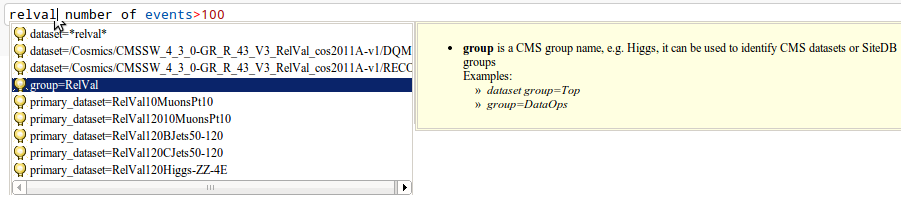
\includegraphics[width=27cm]{images/autocompl.png}
    }
  %% the coordinate (currenty) is used in the default placing of the next blocknode
  %\getcurrentrow{note}
  \getcurrentrow{note}
  \coordinate (currenty) at ($(currentrow)-(yshift)+(xshift)$);

  %%%%%%%%%% ------------------------------------------ %%%%%%%%%%


  \calloutblock[0]{($(kws_north)+(14,-5.5)$)}%
  		{($(currenty)-(7.5,0)$)}{25} %
  {%    
    %\vspace{-0.3cm}
    \textbf{Tokenized query:} 'relval', 'number', 'of', 'events>100'
    }

  \getcurrentrow{note}
  \coordinate (currenty) at ($(currentrow)-(yshift)+(xshift)$);

  %%%%%%%%%% ------------------------------------------ %%%%%%%%%%


  \calloutblock[0]{($(kws_north)+(14,-15.5)$)}%
  		{($(currenty)-(7.5,0)$)}{25} %
  {%    
\vspace{-0.5cm}
    \textbf{Entry points:}\newline
    \input{./entry_points}
        \vspace{-0.3cm}

    }

  \getcurrentrow{note}
  \coordinate (currenty) at ($(currentrow)-(0, 0)+(xshift)$);


  %%%%%%%%%% ------------------------------------------ %%%%%%%%%%
  \blocknode {Future work}%
  {
    %% LyX 2.0.6 created this file.  For more info, see http://www.lyx.org/.
%% Do not edit unless you really know what you are doing.
\documentclass{standalone}
\usepackage{color}
\definecolor{note_fontcolor}{rgb}{0.80078125, 0.80078125, 0.80078125}

\makeatletter

%%%%%%%%%%%%%%%%%%%%%%%%%%%%%% LyX specific LaTeX commands.
%% The greyedout annotation environment
\newenvironment{lyxgreyedout}
  {\textcolor{note_fontcolor}\bgroup\ignorespaces}
  {\ignorespacesafterend\egroup}

\makeatother

\begin{document}

\paragraph*{\vspace{-3cm}}
\begin{itemize}
\item \textbf{advanced autocompletion {[}photo!{]}}
\item improve the ranker
\item look into advanced methods of generic performance improvements to
the services like ``materialized view with the incremental refresh''
\end{itemize}

\paragraph{\textsc{top-K (semi-)optimal solutions with contextualization?}}

\begin{lyxgreyedout}
(only ideas for now...):%
\end{lyxgreyedout}

\begin{itemize}
\item maybe Ranked (Murty\textquoteright{}s) Munkres with Contextualization!?

\begin{itemize}
\item this would at least guarantee optimal top-k for with \textbf{some}
contextualization
\end{itemize}
\item \textbf{out of scope, ask for handouts}
\end{itemize}

\paragraph{\textsc{Reflections on the HMM approach:}}
\begin{itemize}
\item what is modelled is not same as seen by user

\begin{itemize}
\item models $kw_{i}\rightarrow t_{j},$ while user sees structured queries
\item therefore, hard to get automatically collect training data \end{itemize}
\end{itemize}

\end{document}

  }



%  \plainblock[0]{($(box.south east)-(yshift)+(-5,0)$)}%
%  {8cm}{} %
%  {\newline\vspace{-0cm}
%  	\textbf{More info:}\vspace{0.5cm}
%  	\newline
%    
\includegraphics[width=5cm]{images/qrcode.png}
%  	\vspace{-0cm}
%  }  
%    


\end{tikzpicture}


\end{document}




